\chapter{Descripción del Trabajo}
\label{cap:descripcionTrabajo}

\section{Elección del modelo}

Como hemos podido ver, Stable Diffusion es una herramienta potente y eficaz con una buena estructura que cuenta con una gran base de datos en la que podemos encontrar una inmensa variedad de imágenes. Estas características la convirtieron en nuestra elección final, pero veamos más en profundidad el proceso de elección de esta Inteligencia Artificial generativa en comparación con la amplia variedad de las que hay presentes actualmente en el mercado. 

En primer lugar, para entender nuestra elección es necesario poner en contexto el gran abanico de posibilidades de IAs generativas que hay hoy en día, sus prestaciones, características, y sobre todo, su accesibilidad. 

Las IAs generadoras de imágenes más potentes del mercado y las que consideramos para desarrollar la base de nuestro trabajo son Midjourney, DALL-E, Leonardo AI y Stable Diffusion, todas ellas producen unos resultados bastante satisfactorios. Sin embargo, descartamos rápidamente las dos primeras: Midjourney producida por un laboratorio independiente y,
DALL-E producida por la famosa empresa creadora de ChatGPT, OpenAI. El motivo fue que al ser ambas de pago, no podíamos tener acceso a su modelo de forma tan amplia como las demás, siendo prácticamente imposible acceder a ellas y mucho menos a poder entrenarlas. 

Para acceder a los modelos utilizamos Hugging Face, la plataforma  que cuenta con una amplia gama de bases de datos de todo tipo y de modelos de IA generativa de texto a imagen, imagen a imagen, imagen a texto y un largo etcétera. Intentamos buscar modelos de ambas en la plataforma sin éxito ya que lo máximo que encontramos eran imitaciones o pequeñas demos que no alcanzaban el nivel de calidad requerido. \\


Leonardo AI sí que es una opción algo más accesible ya que la plataforma sí que cuenta con un plan gratuito que te deja probar el modelo con una limitación de 150 imágenes a generar al día, lo cual está muy bien. Además, la calidad es bastante buena y permite ajustar gran variedad de parámetros, como por ejemplo, el número de imágenes que deseamos que se generen al mismo tiempo, el estilo, la paleta de colores que deseamos, tamaño e incluso la resolución. El inconveniente era la accesibilidad al modelo y la información sobre este mismo, ya que era escasa y en Hugging Face no había acceso. En comparación con Stable Diffusion, la incertidumbre era mucho más alta y había muchísimas limitaciones a la hora de utilizarlo. \\

Todo ello nos llevó a elegir Stable Diffusion rápidamente, una herramienta open source, es decir, de código abierto que nos facilita mucho el entrenamiento de personas para obtener imágenes personalizadas de forma rápida y con alta calidad. Además, sus diferentes versiones nos permitían explorar aún más a fondo el modelo y saber cuál era el que encajaba con las características que presentaban las prestaciones de nuestros equipos. Stable Diffusion resultó ser la candidata ideal para que la creación de imágenes destinadas a  los libros de vida fuera lo más sencilla, familiar y creativa posible. \\

Ahora expuestos todos los motivos de elección de Stable Diffusion, tanto en comparación con otras redes neuronales vistas en el Capitulo 2 como en comparación con otros modelos de IA Generativa, expondremos cómo implementamos la herramienta a lo largo de todo el trabajo y las dificultades a las que nos enfrentamos durante el proceso. \\

\section{Entrenamiento con Stable Diffusion}

Stable Diffusion cuenta, hasta el momento, con 3 grandes versiones que, paulatinamente, han ido mejorando la calidad en las imágenes generadas. Todas ellas son totalmente gratuitas y de libre acceso, la primera versión que se presentó fue Stable Diffusion 1 (en sus variaciones 1.4 y 1.5), seguida por Stable Diffusion 2 (con sus respectivas variaciones 2.0 y 2.1) y por último, Stable Diffusion XL (que cuenta con su variación XL Turbo). 

La diferencia principal entre las dos primeras versiones es el tamaño de resolución de las imágenes ya que las primeras versiones trabajaban en un espacio de 512x512 píxeles y en la versión 2 dicho tamaño aumentó a 768x758. Además, se introdujeron algunas correcciones y mejoras como la técnica de inpainting, que se trata de la restauración de algunas partes de la imagen mejorando la calidad y los detalles de la misma o incluso, reemplazando ese área por lo especificado por el usuario en el prompt.

Con la última versión Stable Diffusion XL, se generan imágenes con una calidad excepcional, lo que supuso una gran mejora en el modelo al contar con un dataset mucho más extenso. El inconveniente con la versión XL, en nuestro caso, era la limitación de que requiere una tarjeta gráfica demasiado potente, con la que, por desgracia, no contamos en nuestro equipo. 

Respecto a la versión 2, si bien es verdad que no requiere tanta GPU como la versión XL, sí que requiere más que en la primera versión, al ser las imágenes con mayor resolución y, viendo la comparación en la calidad que presentaban los resultados de ambas, optamos por utilizar la versión 1.5 ya que era la que mejor se adecuaba a nosotros en términos de calidad y tiempo.


Ahora bien, existen varios métodos a través de los cuales se puede utilizar esta herramienta y hemos probado sus funcionalidades de diferentes maneras. En primer lugar, se puede utilizar mediante código escrito en Python a través de Google Colab, ya que la plataforma ofrece cuadernos en los que se trabaja de manera online y que además, proporciona una GPU en la nube a la que Google te da acceso. En concreto, esta GPU es la T4, que es la única opción que nos deja Google entre las que hay (A100 GPU, L4 GPU, V100 GPU) ya que se conoce que las demás son de pago. Otra alternativa es mediante la propia página de Stable Diffusion, que ofrece una demo para utilizar esta avanzada versión. Por último, ejecutar el modelo en local, consiguiéndolo descargar en la página Hugging Face, que incluye multitud de modelos de todo tipo, bases de datos, librerías y licencias para descargar y utilizar, por lo que hemos podido comprobar,presenta muy buenos resultados.\\

El hecho de probar un modelo de inteligencia artificial en un servidor no es concordante con nuestros objetivos del proyecto, puesto que necesitamos entrenar un modelo e incluirlo en una aplicación, de manera que el usuario pueda interactuar y conseguir imágenes personalizadas en un tiempo aceptable, por ello descartamos la opción de utilizar la demo que se encuentra en la página de Stable Diffusion. \\

Una vez que tenemos el modelo de generación de imágenes elegido, se debe ejecutar en nuestro ordenador y ver cuál es el rendimiento real. Esto quiere decir que la imagen debe generarse de manera correcta y sin deformaciones, y debe incluir todos los elementos solicitados en la descripción introducida. Además, debe realizar esta generación en un tiempo adecuado.\\

Para ello, el proceso más óptimo y que finalmente elegimos llevar a cabo tras gran cantidad de pruebas es, en primer lugar, realizando el entrenamiento de imágenes personales a través de la plataforma de Google Colab en internet y en segundo lugar, para la generación de imágenes desde nuestro ordenador optamos por la instalación de una interfaz, llamada NMKD Stable Diffusion GUI. Esta herramienta nos permite ejecutar localmente cualquier modelo de generación de imágenes a partir de texto, e incluso permite aceptar imágenes como input, es decir, generaciones de tipo imagen a imagen. 

El principal de los objetivos que establecimos en la realización del proyecto era generar imágenes personalizadas del paciente en cuestión, y para ello es estrictamente necesario entrenar el modelo elegido.

Como se ha dicho anteriormente, el método elegido fue un cuaderno en Google Colab mediante Dreambooth,  un modelo de generación de aprendizaje profundo, y que fue desarrollado en 2022 por un grupo de investigadores de Google Research y la Universidad de Boston.  Este modelo nos permite añadir capas de entrenamiento a la inteligencia artificial para que reconozca objetos concretos. Esto es muy importante, porque es el mecanismo que consigue mejores resultados y con una velocidad aceptable, que era la utilización que queríamos otorgarle. Por consiguiente, podemos decir que la misión de esta tecnología es la de poder entrenar a modelos de inteligencia artificial para personalizarlo según tus necesidades.

Para realizar el entrenamiento de una forma correcta, lo primero que tenemos que tener claro es  el elemento o token al que queremos dar una identidad. Por ejemplo, si seleccionamos una persona, debemos elegir unas imágenes en las que aparezca, de tal manera que, tras el entrenamiento, la IA pueda identificarla. 

Lo ideal es que se elija un número considerable de fotografías, a partir de 10, las cuales tienen que cumplir ciertas características. Deben ser fotografías de buena calidad, bajo diferentes ángulos, escenarios y luces, se recomienda que como mínimo hayan 1 o 2 fotografías en las que la persona aparezca de perfil, mostrando 3 cuartos de la cara, de frente y si es posible que en alguna esté sonriendo (para que la IA pueda reconocer la expresión), de cuerpo entero, cintura para arriba y del rostro de cerca. Además, es importante que la ropa no sea siempre la misma, sino al ser así, el modelo podría interpretar como que la ropa forma parte de la persona y siempre se la generaría con la misma, lo cual no queremos que ocurra. Idealmente, las fotografías deberían alternar la luz y estar hechas tanto en interiores como en exteriores. Por último y esto es fundamental, estas deberán tener un tamaño igual o mayor a 512 x 512 píxeles, y deberán llamarse exactamente de la misma manera, con el identificador del token al que hagamos referencia. Además, es preferible que todas las imágenes tengan la misma extensión, ya sea .jpg o .png. 

En el ejemplo de la figura \ref{fig:datasethoyeon}  elegimos como persona de entrenamiento una que no fuese reconocida por nuestro modelo (al contar con un dataset de 5 mil millones de imágenes, ya de por sí reconoce a varias personas famosas sin necesidad de entrenarlas). En este caso, se trata de una actriz coreana llamada Jung Hoyeon, y el token que le otorgamos, como se puede ver, respondía bajo el nombre de "sqgkhoju". Lo ideal, es que la etiqueta no sea nombrada bajo una palabra que el modelo pueda reconocer, es decir, que el token no tenga significado. Si por un casual llamasemos al token "mujer", seguramente la IA no logre ni identificar ni asociar a la persona que hemos entrenado, y probablemente acabe generando la imagen de una mujer que no existe, que es justamente lo que queremos evitar. \\

\begin{figure}[h]
	\centering
	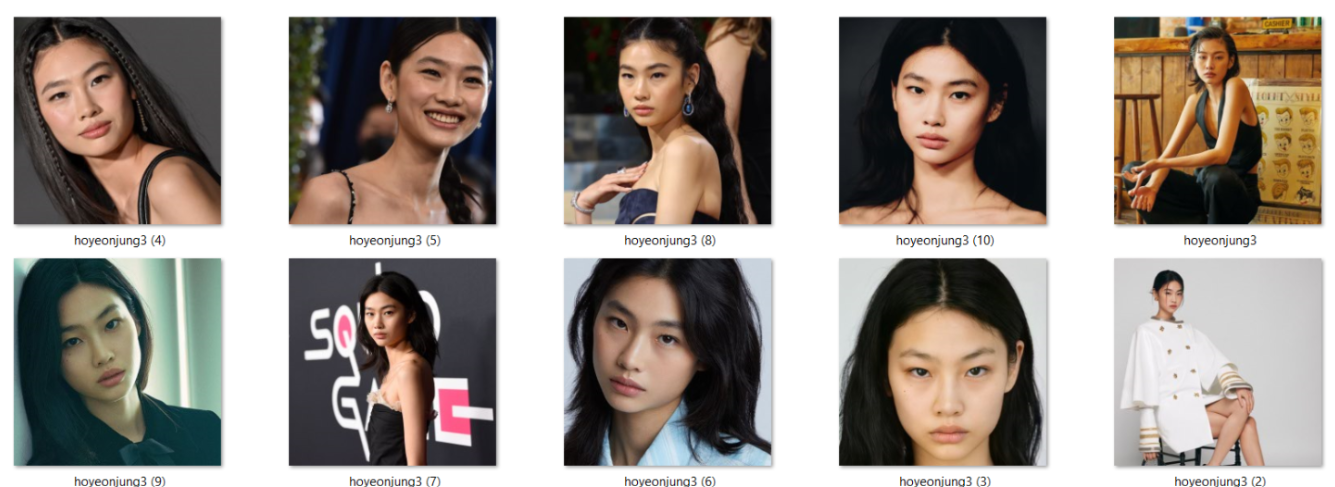
\includegraphics[width = 1
	\textwidth]{Imagenes/Vectorial/datasethoyeon.png}
	\caption{Dataset seleccionado para el entrenamiento de personas con Lora}
	\label{fig:datasethoyeon}
\end{figure}

Una vez que las imágenes cumplan con todos los requisitos, debemos utilizar el código abierto en la plataforma Google Colab para realizar el entrenamiento. 
El proceso que sigue el cuaderno es muy sencillo, en él sólo hace falta seguir una serie de pasos para completarlo. El primero es conectar el cuaderno a una cuenta de Google, para que se pueda guardar en el Drive asociado a esa cuenta una carpeta llamada "Fast-Dreambooth", en la que se guardaran todos los archivos que se generen durante el proceso. El siguiente paso es instalar las dependencias necesarias para ejecutar el código en python, seguido de establecer un nombre a la sesión en la que estamos trabajando, para que en un futuro cuando se hagan entrenamientos diferentes, se puedan distinguir unos de otros. En este paso se crea una carpeta llamada Sessions dentro de la carpeta mencionada recientemente. A su vez, esta carpeta contendrá otra bajo el nombre de la sesión que hayamos especificado en el cuaderno, y es ahí donde se guardaran todos los archivos que se creen en la ejecución. 

A continuación, es turno de subir las imágenes previa y cuidadosamente seleccionadas. Ya sea seleccionándolas directamente desde la carpeta en la que las tengamos guardadas en local, o habiéndolas subido previamente a una carpeta de la cuenta de Google Drive, y proporcionar la ruta en la que están en la celda del cuaderno habilitada para ello. 

El último paso, y uno de los más importantes, consiste en establecer algunos parámetros con los que se va a entrenar al modelo. El más importante y el único que nosotros hemos modificado, entre todos los que hay, es el número de steps. De modo que, en cuanto mayor sean, más tiempo tardará en generarse el archivo. Normalmente, se tardaba unos 20 o 25 minutos en terminar de entrenarse, lo cual hemos considerado que es bastante rápido. En el ejemplo de la figura \ref{fig:dreambooth} se puede ver la ejecución del progreso de entrenamiento en el que para una cantidad de 2000 pasos lleva 21 minutos y 36 segundos. 

Tras la finalización, se creará un archivo de alrededor de 2 giga bytes, que contendrá el modelo de Stable Diffusion 1.5, con una capa de entrenamiento más, puesto que incorporará el elemento deseado. Con esto ya tendríamos un elemento de inteligencia artificial personalizado.\\

\begin{figure}[h]
	\centering
	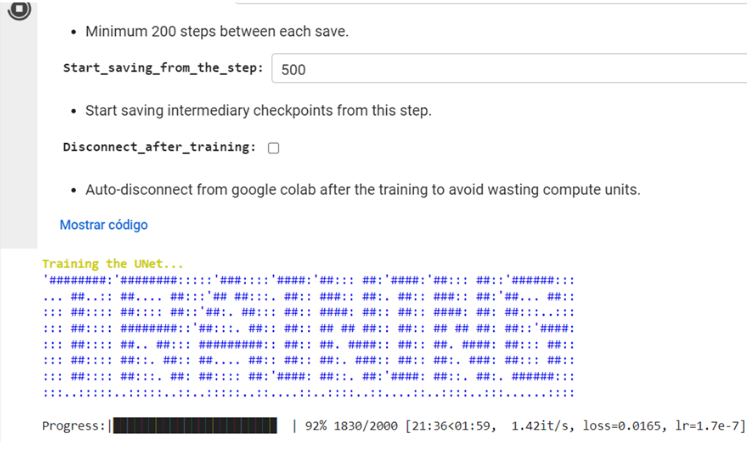
\includegraphics[width = 1
	\textwidth]{Imagenes/Vectorial/dreambooth.png}
	\caption{Procedimiento del entrenamiento mediante Dreambooth}
	\label{fig:dreambooth}
\end{figure}

Este archivo, en formato ckpt, se podrá utilizar en la aplicación SKMD GUI más adelante para generar imágenes, y contendrá el elemento entrenado bajo el token seleccionado. Si posteriormente se pretende incluir elementos al modelo ya entrenado, también se puede realizar empezando de nuevo el proceso de entrenamiento y utilizando de base el archivo en extensión ckpt anterior. Cuando se realice este segundo entrenamiento, se podrán generar imágenes acerca de ambos elementos, lo cuál es muy útil para nuestros objetivos, ya que en un mismo modelo enfocado a un paciente, debe haber múltiples elementos. Sin embargo, más adelante veremos que este último aspecto ha supuesto uno de los grandes fallos que experimenta el modelo en cuanto a múltiples capas de entrenamiento. \\

Un aspecto muy importante a tener en cuenta, es que tras la realización de múltiples pruebas, los resultados óptimos que hemos obtenido ha sido seleccionando un conjunto de datos formado por 10 imágenes, y con 2400 pasos de entrenamiento. En la tabla \ref{tab:resultadosentrenamiento}\\


\begin{table}
	\centering
	\begin{tabular}{c|c|c|c}
		\textbf{Intento} & \textbf{Número de imágenes} & \textbf{Número de pasos} & \textbf{Veredicto} \\
		\hline\hline
		1 & 20 & 4000 & \\
		2 & 20 & 3000 & \\
		3 & 15 & 3000 & \\
		4 & 15 & 2000 & \\
		5 & 10 & 3000 & \\
		6 & 10 & 2400 & \\
		\hline
	\end{tabular}
	\caption{Tabla de resultados obtenidos de entrenamiento}
	\label{tab:resultadosentrenamiento}
\end{table}



Hemos querido poner a prueba, no sólo las capacidades del modelo de entrenar a personas, ya que hemos podido comprobar sus puntos fuertes y débiles en la generación de seres humanos (los cuales podremos ver más adelante), sino de elementos que consideramos que también son de suma importancia a la hora de representar recuerdos: animales y lugares. 

El objetivo de entrenar al modelo con lugares es que estos no se encuentren en la base de datos de imágenes de Stable Diffusion, puesto que de ser así, no tendría sentido realizar el entrenamiento. De este modo, podremos lograr que el paciente pueda rememorar sitios emblemáticos para él o ella y que las imágenes generadas que emulan recuerdos consigan ser aún más personales. Por ejemplo, el parque de su vecindario, la casa de sus padres o incluso, su propio salón. 

Las primeras pruebas que realizamos sobre un lugar se trataba de un edificio característico, que por supuesto no estaba incluido previamente. Hablamos de la basílica de Colmenar Viejo, Madrid. Las imágenes seleccionadas estaban hechas desde diferentes ángulos, alturas, luces y lejanías. En la figura \ref{fig:datasetcolme} se pueden apreciar las características que reúnen las fotografías en cuestión y el token otorgado.

Además, quisimos comprobar si el número de imágenes y steps establecidos para las personas, producía resultados igual de satisfactorios para lugares. Y efectivamente, corroboramos la hipótesis de manera airosa. Ejemplos de ello, lo podemos ver en el apartado siguiente.  

\begin{figure}[!htb]
	\centering
	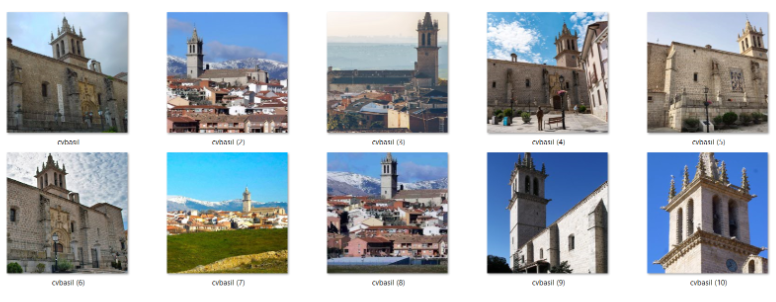
\includegraphics[width = 1
	\textwidth]{Imagenes/Vectorial/dataset_colmenar.png}
	\caption{Dataset seleccionado para el entrenamiento con lugares}
	\label{fig:datasetcolme}
\end{figure}

Para el entrenamiento de animales, seleccionamos 10 fotografías de un perro de la raza Shiba Inu en diferentes perspectivas, escenarios y mostrando distintas emociones para comprobar si la inteligencia artificial permitía entrenar con animales. Sin embargo, a la luz de los resultados vistos en personas y lugares quisimos comprobar la técnica de LORA que presenta Stable Diffusion. Las siglas LORA hacen referencia a \textit{Low-Rank Adaptation of Large Language Models}, del inglés. Esta técnica favorece un equilibrio entre el tamaño del archivo y la eficiencia del propio entrenamiento y como vimos en el Capítulo 2 del Estado de la Cuestión, ha presentado imágenes de gran calidad en un tiempo excepcional.

El hecho de cambiar a LORA no supuso grandes cambios a la hora de entrenar el elemento deseado debido a que la selección de imágenes es exactamente igual. Donde realmente cambia el entrenamiento es en el cuaderno utilizado en Google Colab, este es diferente y por lo tanto, la forma de ejecución y los pasos a seguir también lo son. 


Es de vital importancia saber cuáles son los parámetros que se deben ajustar para poder desarrollar el modelo de manera correcta y entender cada uno de ellos, dado que pueden resultar un poco más complejos en comparación con la técnica del cuaderno de Fast-Dreambooth.\\

*****************************************************************************************************
Se debe indicar el nombre del proyecto. Es muy importante, porque  aquí es donde obtendremos el resultado final, y es donde se debe incluir el dataset que mencionamos en el párrafo anterior. A continuación, el modelo a entrenar, como se ha explicado, hemos elegido el Stable Diffusion 1.5, por lo que es el que sirve de base para todos los entrenamientos escogidos. No obstante, esta técnica de entrenamiento tiene la peculiar característica de que se puede utilizar de base cualquier checkpoint desarrollado previamente, por lo que en caso de realizar un entrenamiento sobre personas, existe la posibilidad de elegir un modelo de base especializado en retratos. Esto garantiza que, seleccionando unas fotografías adecuadas y ajustando de manera correcta cada parámetro, los resultados sean bastante buenos.\\

Animales:\\
Para realizar una prueba del modelo de entrenamiento con Lora, lo primero fue elegir el animal y crear nuestro propio conjunto de datos, de manera que había que escoger 10 imágenes que tuviesen un tamaño igual o superior a 512 x 512 píxeles, y que la relación entre el ancho y el alto fuese 1 a 1. Además, al elegir el animal, se hizo la comprobación de que Stable Diffusion no lo incorporara ya en el modelo.\\ 

\begin{figure}[h]
	\centering
	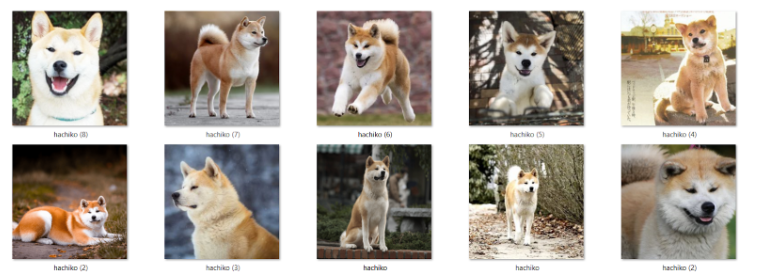
\includegraphics[width = 1
	\textwidth]{Imagenes/Vectorial/dataset_hachiko.png}
	\caption{Dataset seleccionado para el entrenamiento con animales}
	\label{fig:datasethachi}
\end{figure}

Como se puede apreciar en la figura anterior, se hizo hincapié en la diversidad de las imágenes, para aportar un mayor valor al entrenamiento, de modo que se tuviese una visión completa del elemento a entrenar.\\

*******************************************************


Ahora podemos decir que hemos logrado entrenar un modelo de generación de imágenes incluyendo fotografías propias, y eso es algo que puede ser realmente útil para nuestros siguientes propósitos. Esto es porque podemos lograr que cualquier persona pueda incorporar las imágenes que considere oportunas para servir de apoyo al paciente. Lo cual consideramos un éxito en el desarrollo de nuestro trabajo. 


\section{Generación de imágenes con la interfaz de Stable Diffusion}

\subsection{Requisitos de instalación}

La instalación se realizó desde el siguiente link 
https://nmkd.itch.io/t2i-gui

OS: Windows 10/11 64-bit

Minimum:
GPU: Nvidia GPU with 4 GB VRAM, Maxwell Architecture (2014) or newer

Alternatively, with limited feature support: Any DirectML-capable GPU with 8 GB of VRAM
RAM: 8 GB RAM (Note: Pagefile must be enabled as swapping will occur with only 8 GB!)

Disk: 10 GB (another free 5 GB for temporary files recommended)

Recommended:
GPU: Nvidia GPU with 8 GB VRAM, Pascal Architecture (2016) or newer
RAM: 16 GB RAM
Disk: 12 GB on SSD (another free 5 GB for temporary files recommended)

\textbf{**explicar extensamente los requisitos que se deben cumplir para instalarse la app (GPU, cuda, memoria y etc)}

\subsection{Funcionamiento y detalles de la interfaz}

 
para que sirven los botones y ajustes etc

**explicar como funciona para integrar diferentes modelos, loras, establecer los parametros a la hora de generar la imagen

\subsection{Resultados de generación de imágenes}



Para la ejecución, debemos seleccionar un modelo , introducir una descripción y ajustar el número de pasos, que determinarán la duración de la generación y la calidad de la imagen, en función del modelo escogido y las limitaciones que presenta la tarjeta gráfica, que como hemos explicado es fundamental para esta tarea. Uno de los puntos a favor de esta interfaz, y que resulta de gran interés para nuestro proyecto, es que permite la utilización de modelos personalizados. \\

Para la personalización del modelo de Stable Diffusion hemos probado distintas vías y se ha llegado a distintos resultados y conclusiones:\\



 
Una vez entrenado el modelo, obtuvimos un total de 10 archivos en formato safetensor. Esto es debido a que, como hemos explicado con anterioridad, Lora tiene la ventaja de devolver múltiples resultados con un número de pasos distinto, con el objetivo de tener la posibilidad de probar cuáles son los steps ideales, y con cuáles habría falta o exceso de entrenamiento. En este caso, el safetensor adecuado fue el primero, puesto que a partir del segundo se podía apreciar la deformidad típica del sobreentrenamiento.\\
\begin{figure}[h]
	\centering
	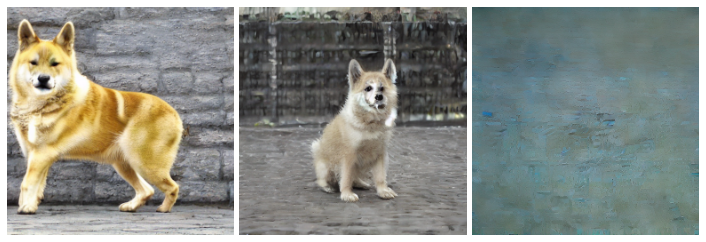
\includegraphics[width = 0.6
	\textwidth]{Imagenes/Vectorial/comparacion_hachiko.png}
	\caption{Mismo prompt con 1000, 2000 y 10.000 pasos de entrenamiento}
	\label{fig:comphachi}
\end{figure}

En el momento en el que se descartan los demás archivos Safetensor, la siguiente labor es probar cuál es el número de pasos ideal para la generación de imágenes, y descubrir si con diferentes prompts, el modelo entrenado podría obtener buenos resultados.\\


**explicar mejor


\begin{figure}[h]
	\centering
	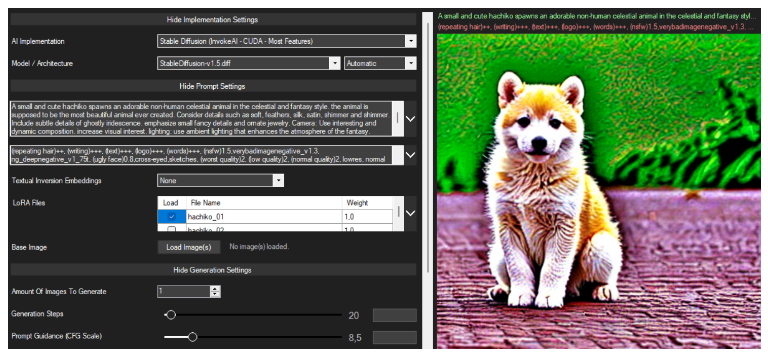
\includegraphics[width = 0.6
	\textwidth]{Imagenes/Vectorial/hachiko_detallada.png}
	\caption{Imagen generada con el modelo Stable Diffusion 1.5, Lora Hachiko}
	\label{fig:detallehachi}
\end{figure}



\begin{figure}[h]
	\centering
	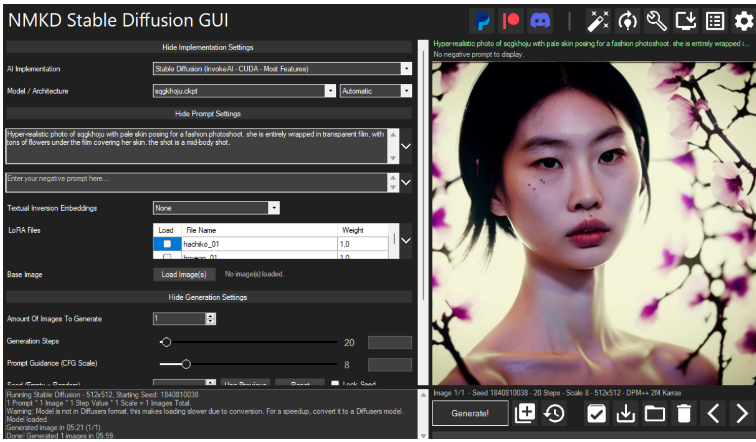
\includegraphics[width = 0.5
	\textwidth]{Imagenes/Vectorial/hoyeon1.png}
	\caption{Resultados de entrenamiento de una persona con Dreambooth}
	\label{fig:hoyeonsd}
\end{figure}

\begin{figure}[h]
	\centering
	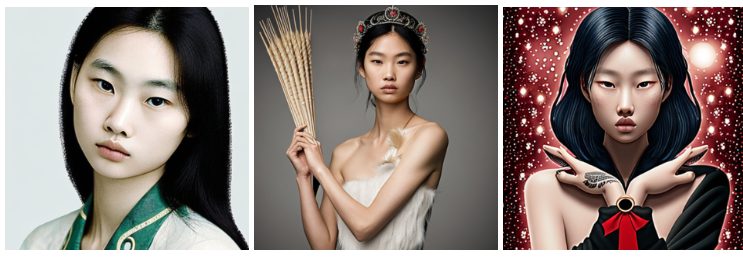
\includegraphics[width = 0.6
	\textwidth]{Imagenes/Vectorial/hoyeon_results.png}
	\caption{Resultados de entrenamiento de una persona con diferentes estilos}
	\label{fig:imagshoyeon}
\end{figure}


Con diferentes estilos:\\

\begin{figure}[!htb]
	\centering
	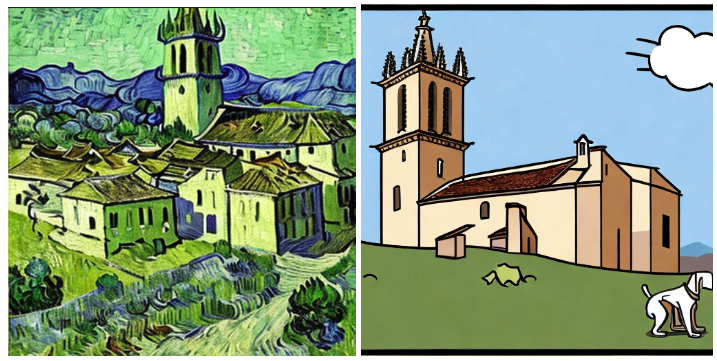
\includegraphics[width = 0.6
	\textwidth]{Imagenes/Vectorial/colmenar_styles.png}
	\caption{Resultados de imagenes del lugar entrenado al estilo Van Gogh y viñeta}
	\label{fig:colmestyles}
\end{figure}


Añadiendo otros elementos:\\


\begin{figure}[!htb]
	\centering
	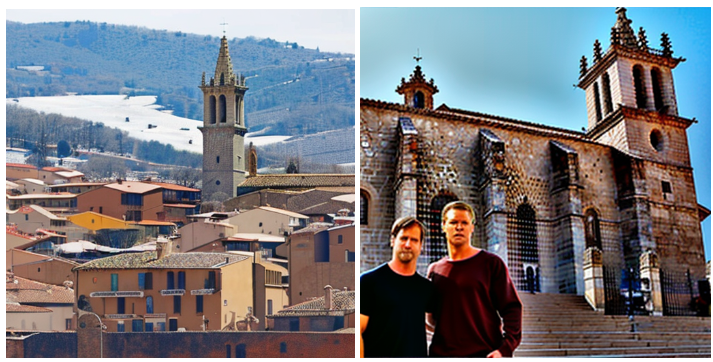
\includegraphics[width = 0.6
	\textwidth]{Imagenes/Vectorial/colmenar_elements.png}
	\caption{Resultados de imágenes del lugar en invierno y con una persona}
	\label{fig:elementscolme}
\end{figure}


Peligros con el sobreentrenamiento: Se produce cuando el modelo no se puede generalizar y se ajusta demasiado al conjunto de datos entrenados. Se debe principalmente a que el tamaño de los datos es demasiado pequeño y no contiene suficientes muestras de datos para poder representar con precisión la totalidad de datos de entrada posibles. Otra razón es que el modelo se entrena durante demasiado tiempo en un solo conjunto de datos de muestra. En nuestro modelo, encontramos sobreentrenamiento cuando elegimos un número de steps muy elevado para un número de fotografías que no es lo suficientemente alto. Una manera de detectar que nuestro modelo está sobreentrenado es cuando no genera bien la cara de la persona, y se aprecian fallos en determinadas facciones, como en los ojos y la boca, en los cuales se aprecia deformidad.\\

Falta de pasos en el entrenamiento: En este caso, se produce cuando el modelo de datos no tiene la capacidad de capturar de forma precisa la relación entre las variables de entrada y de salida, de manera que existe un elevado índice de errores en el conjunto de datos de entrenamiento y en los datos no vistos. Se debe a que el modelo es demasiado simple, porque el tamaño de los datos es demasiado pequeño, o bien porque se necesita más tiempo de entrenamiento. En este caso, cuando generamos las imágenes, se evidencia que el modelo aún no ha aprendido lo suficiente acerca del elemento o token del que se ha realizado el entrenamiento, pues el resultado de la generación refleja una persona que no muestra ningún parecido con la realidad.\\

En cuanto a mezcla de personas: Para ampliar los horizontes de nuestro entrenamiento, hemos entrenado a una persona, asociando un token a ella para su identificación, sobre un modelo que previamente ya había sido entrenado con una persona y su token asociado, para comprobar si efectivamente se podía generar en una sola imagen una representación de las dos personas entrenadas, una junto a la otra. Es aquí donde se ha detectado una peculiaridad, ya que, a pesar de que un modelo genere buenos resultados de cada una de las dos personas, en el mismo momento que se solicita en un determinado prompt o descripción que se vean reflejados una o varias personas entrenadas en la misma fotografía, ningún modelo de los que se haya probado, ha generado buenos resultados de esta manera. Lo que finalmente se aprecia en la imagen generada, es que aparecen dos personas pero sus rostros son una mezcla de las características faciales y fisiológicas de ambas, produciéndose una deformidad en muchos de los casos y que los rostros aparezcan prácticamente duplicados.
\begin{figure}[h]
	\centering
	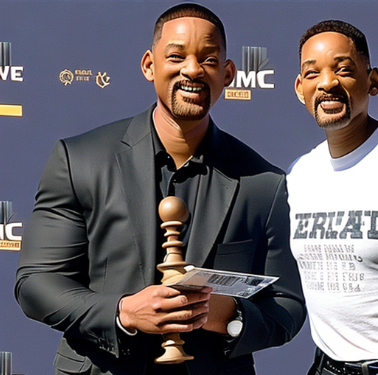
\includegraphics[width = 0.4
	\textwidth]{Imagenes/Vectorial/duplicidad_will.png}
		\caption{Duplicidad de elementos}
	\label{fig:willpor2}
\end{figure}


**sñadir capitulo 4 para el funcioonamiento de la aplicacion

4.1. backend\\

4.2. frontend\\



Avances respecto al modelo.\\

Aplicación de Stable Diffusion genera imágenes aceptables en un tiempo normal (1-2 minutos como máximo). Existe la posibilidad de utilizar imágenes para poder incorporar al modelo de Stable Diffusion como Token. La aplicación contiene un apartado de training, pero tras probar incorporar escasas imágenes al modelo, el proceso es demasiado largo (varios días) y el resultado es una incógnita. \\

El modelo de .csv parece estar obsoleto, y al intentar el entrenamiento con las imágenes de personas sale un error en el paso 6, lo cual limita y habrá que identificar y trabajar con otro modelo de entrenamiento. LoRA puede ser una opción para ello.
También hemos probado más modelos de Hugging Face a ejecutar por consola mediante Anaconda, pero los resultados no son los adecuados. Generan imágenes de calidad no muy buena en un tiempo muy elevado, entre 10 y 20 minutos. Por tanto, también decidimos descartar esta vía. 
La más razonable hasta ahora es la GUI de Stable Diffusion, ya que es la única que genera imágenes en un tiempo adecuado, y que permite la posibilidad de incorporar imágenes propias al modelo\\

